\documentclass[11pt, titlepage]{article}
\usepackage{amsmath,amsthm,amssymb}
\usepackage{hyperref, pgf, tikz}
\usepackage{fancyhdr}
\usetikzlibrary{arrows}
\usepackage[margin=1.25in]{geometry}
\usepackage{graphicx}     
\usepackage{sidecap}                
\pagestyle{fancy}
\usepackage{array}
\usepackage{multirow}

\lhead{Lab \#03}
\rhead{\thepage}
\cfoot{}

\title{\Huge{The Addition and Resolution of Vectors: The Force Table} \\ \ \\ \huge Lab \#03}
\author{\Large{Alon Levin} \\ \emph{Lab Partners: Sophia Zheng, Avery Karlin}}
\date{\today}
\begin{document}

\maketitle

\begin{center}
\LARGE The Addition and Resolution of Vectors: The Force Table
\end{center}

\section*{Objective}
The objectives of this lab are to learn two methods of adding sets of vectors (graphically and analytically) and thus to foster an appreciation of the differences between the two approaches.

\section*{Introduction}
A \textbf{vector} is a mathematical concept which represents a quantity that has both a magnitude and a direction, unlike a \textbf{scalar} which has only a magnitude. Therefore, the process of adding vectors is more complex as well; there are three ways to find a vector sum: graphically, analytically, or experimentally.

\subsection*{Graphical Methods}
Vectors are represented graphically as arrows, with the length proportional to the magnitude and the direction represented by the direction the arrowhead points in. As can be seen in Fig. \ref{fig:1}, the graphical method can be approached in three ways.
\begin{figure}[!ht]
\centering
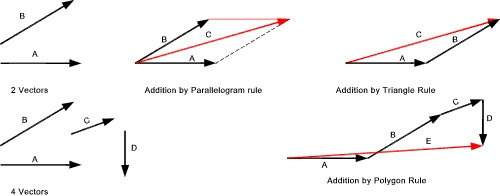
\includegraphics[scale=1, angle=0]{lab03_graphicvectors.jpg}
\caption{Three methods for graphical vector addition \label{fig:1}}
\end{figure} 
\begin{description}
	\item[Parallelogram] Given two vectors $\mathbf{A ~\text{and} ~B}$, a parallelogram could be constructed with $\mathbf{A} ~\text{and} ~\mathbf{B}$ as adjacent sides. The arrow diagonal of the parallelogram $\mathbf{R}$ is the resultant of $\mathbf{A} + \mathbf{B}$. In Fig. \ref{fig:1}, $\mathbf{R} ~\text{is denoted as} ~\mathbf{C}$.
	\item[Triangle] Given two vectors $\mathbf{A ~\text{and} ~B}$, the ``tail'' of $\mathbf{B}$ could be attached from the ``head'' of $\mathbf{A}$. The vector drawn from the tail of $\mathbf{A} ~\text{to the head of} ~\mathbf{B}$ is the resultant $\mathbf{R}$ of $\mathbf{A} + \mathbf{B}$. In Fig. \ref{fig:1}, $\mathbf{R} ~\text{is denoted as} ~\mathbf{C}$.
	\item[Polygon] For situations in which more than two vectors are added, the ``head-to-tail'' method employed in the \textbf{Triangle rule} can be employed repeatedly to form a polygon constructed of vectors. In Fig. \ref{fig:1}, $\mathbf{R} ~\text{is denoted as} ~\mathbf{E}$.
\end{description}

\subsection*{Analytical Methods}
The concept of a vector's magnitude and direction allow for more accurate mathematical methods of calculating vector sums.
\begin{figure}[!ht]
\centering
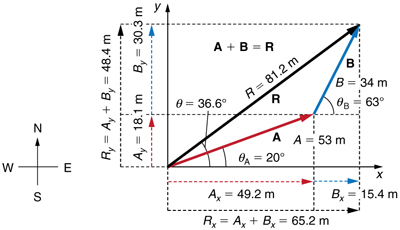
\includegraphics[scale=1.5, angle=0]{lab03_analyticalvectors.jpg}
\caption{Vector Sum broken into components and angles \label{fig:2}}
\end{figure} 

\noindent The components of a vector $\mathbf{V}$, with magnitude $V$ and angle $\theta$, are defined as
$$ V_x = V \cos\theta$$
\begin{equation} \label{eq:1}
V_y = V \sin\theta
\end{equation}
As shown by Fig. \ref{fig:2}, after vectors $\mathbf{A} ~\text{and} ~\mathbf{B}$ are placed head-to-tail, the values of their components and angles can be used in various ways to obtain the final values of the resultant $\mathbf{R}$'s magnitude and angle. To find the components, magnitude, and direction of $\mathbf{R}$, the following formulas are used:
$$R_x = A_x + B_x$$
$$R_y = A_y + B_y$$
$$R = \sqrt{R_x^2 + R_y^2}$$
\begin{equation} \label{eq:2}
\theta = \arctan({\frac{R_y}{R_x}})
\end{equation}

\subsection*{Experimental Methods}
A \textbf{force table} (see Fig. \ref{fig:3}) is essentially a circular table with a rim calibrated in degrees. Weight forces are applied to a central ring by means of systems of strings and pulleys, allowing for vectors to be modeled  both in direction (by varying the direction of the string) and in magnitude (by varying the weight pulling down on the string). The equlibirant $\mathbf{E}$ of several vectors can be found by creating an additional vector to balance out the pre-existing vectors. The equilibriant is a vector force of equal magnitude but opposite direction to the resultant; thus, by finding the equilibriant one can easily calculate the resultant $\mathbf{R} = -\mathbf{E}$

\section*{Procedure}
After setting up the force table as shown in Fig. \ref{fig:3}, read the situations given in the problems below. Using all three methods of calculating the resultant, solve the problems and compare the values of $\mathbf{R}$ found using each method.
\begin{figure}[!ht]
\centering
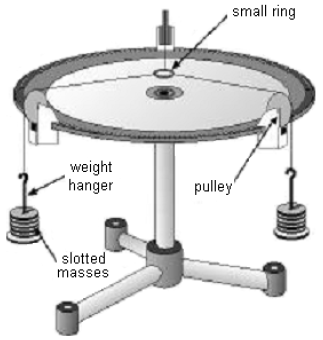
\includegraphics[scale=.65, angle=0]{lab03_forcetable.png}
\caption{Setup of Force Table \label{fig:3}}
\end{figure}

\section*{Data}
\begin{table}[!ht]
\hskip-2.0cm
\begin{tabular}{|c|c|c|c|c|}
\hline
\multirow{2}{*}{}                       & \multirow{2}{*}{Forces (N)}                                               & \multicolumn{3}{c|}{Resultant $\textbf{R}$ (magnitude and direction)}            \\ \cline{3-5} 
                                        &                                                                           & Graphical             & Analytical            & Experimental          \\ \hline
Vector addition 1                       & \begin{tabular}[c]{@{}c@{}}$F_1 = (0.200)g \text{ N, } \theta_1 = 30^\circ$ \\ $F_2 = (0.200)g \text{ N, } \theta_2 = 120^\circ$ \end{tabular} & \begin{tabular}[c]{@{}c@{}}$F = (0.280)g \text{ N}$ \\ $\theta = 75^\circ$ \end{tabular} & \begin{tabular}[c]{@{}c@{}}$F = (0.283)g \text{ N}$ \\ $\theta = 75.0^\circ$ \end{tabular} & \begin{tabular}[c]{@{}c@{}}$F = (0.280)g \text{ N}$ \\ $\theta = 75^\circ$ \end{tabular} \\ \hline
Vector addition 2                       & \begin{tabular}[c]{@{}c@{}}$F_1 = (0.200)g \text{ N, } \theta_1 = 20^\circ$ \\ $F_2 = (0.150)g \text{ N, } \theta_2 = 80^\circ$ \end{tabular}   & \begin{tabular}[c]{@{}c@{}}$F = (0.305)g \text{ N}$ \\ $\theta = 45^\circ$ \end{tabular} & \begin{tabular}[c]{@{}c@{}}$F = (0.304)g \text{ N}$ \\ $\theta = 45.3^\circ$ \end{tabular} & \begin{tabular}[c]{@{}c@{}}$F = (0.300)g \text{ N}$ \\ $\theta = 45.5^\circ$ \end{tabular} \\ \hline
Vector addition 3                       & \begin{tabular}[c]{@{}c@{}}$F_1 = F_x = (0.200)g \text{ N, } \theta_1 = 0^\circ$ \\ $F_2 = F_y = (0.150)g \text{ N, } \theta_2 = 90^\circ$ \end{tabular} & \begin{tabular}[c]{@{}c@{}}$F = (0.250)g \text{ N}$ \\ $\theta = 37^\circ$ \end{tabular} & \begin{tabular}[c]{@{}c@{}}$F = (0.250)g \text{ N}$ \\ $\theta = 36.9^\circ$ \end{tabular} & \begin{tabular}[c]{@{}c@{}}$F = (0.250)g \text{ N}$ \\ $\theta = 38^\circ$ \end{tabular} \\ \hline
Vector resolution                       & $F = (0.300)g \text{ N, } \theta_1 = 60^\circ$            & \begin{tabular}[c]{@{}c@{}}$F_x = (0.150)g ~\text{N}$ \\ $F_y = (0.260)g ~\text{N}$ \end{tabular}   & \begin{tabular}[c]{@{}c@{}}$F_x = (0.150)g ~\text{N}$ \\ $F_y = (0.260)g ~\text{N}$ \end{tabular} & \begin{tabular}[c]{@{}c@{}}$F_x = (0.160)g ~\text{N}$ \\ $F_y = (0.260)g ~\text{N}$ \end{tabular} \\ \hline
Vector addition 4                       & \begin{tabular}[c]{@{}c@{}}$F_1 = (0.100)g \text{ N, } \theta_1 = 30^\circ$ \\ $F_2 = (0.200)g \text{ N, } \theta_2 = 90^\circ$ \\ $F_3 = (0.300)g \text{ N, } \theta_3 = 225^\circ$ \end{tabular} & \begin{tabular}[c]{@{}c@{}}$F = (0.130)g \text{ N}$ \\ $\theta = 163^\circ$ \end{tabular} & \begin{tabular}[c]{@{}c@{}}$F = (0.131)g \text{ N}$ \\ $\theta = 163.2^\circ$ \end{tabular} & \begin{tabular}[c]{@{}c@{}}$F = (0.120)g \text{ N}$ \\ $\theta = 156^\circ$ \end{tabular} \\ \hline
\end{tabular}
\caption{Results of vector addition (note: $g = 9.81 \frac{m}{s^2}$)}
\end{table}

\section*{Graphical Analyses}
\begin{SCfigure}[][!ht]
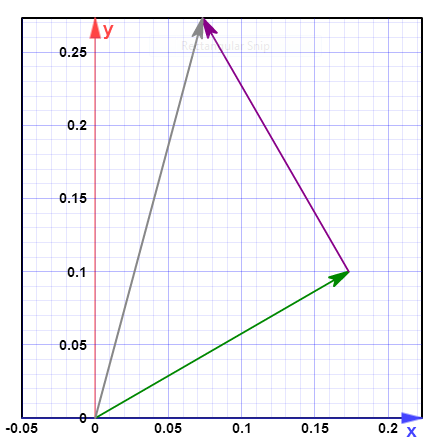
\includegraphics[scale=.5, angle=0]{lab03_v1.png}
\caption{Vector Addition 1 \label{fig:v1}}
\end{SCfigure}
\begin{SCfigure}[][!ht]
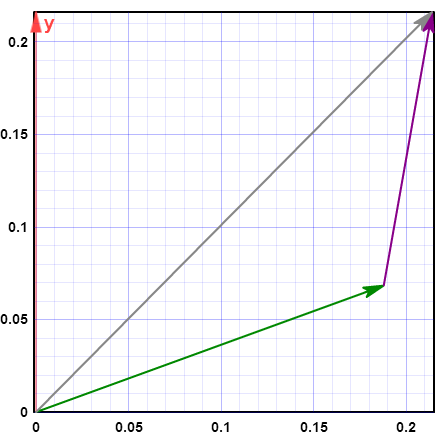
\includegraphics[scale=.5, angle=0]{lab03_v2.png}
\caption{Vector Addition 2 \label{fig:v2}}
\end{SCfigure}
\begin{SCfigure}[][!ht]
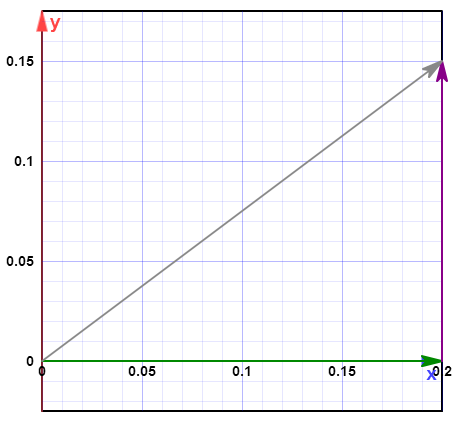
\includegraphics[scale=.5, angle=0]{lab03_v3.png}
\caption{Vector Addition 3 \label{fig:v3}}
\end{SCfigure}
\begin{SCfigure}[][!ht]
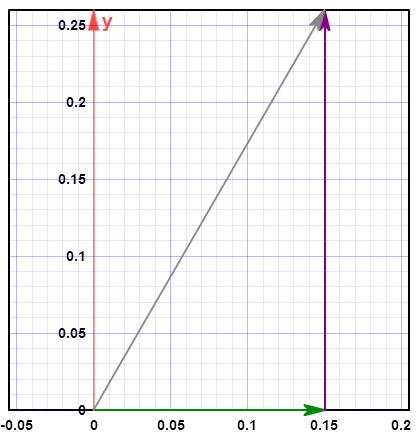
\includegraphics[scale=.5, angle=0]{lab03_v4.png}
\caption{Vector Resolution \label{fig:v4}}
\end{SCfigure}
\begin{SCfigure}[][!ht]
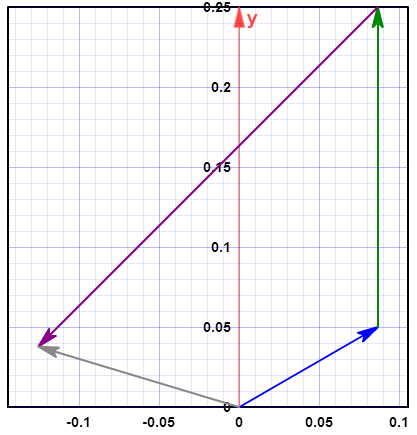
\includegraphics[scale=.5, angle=0]{lab03_v5.png}
\caption{Vector Addition 4 \label{fig:v5}}
\end{SCfigure}

\pagebreak
\section*{Discussion}
\subsection*{Sample Calculations}
Using Eqs. \ref{eq:1} and \ref{eq:2} for Vector Addition 1:
$$F_x = F_{1x} + F_{2x} = F_1\cos\theta_1 + F_2\cos\theta_2 = .2g\cos(30^\circ) + .2g\cos(120^\circ) = 0.073g \text{ N}$$
$$F_y = F_{1y} + F_{2y} = F_1\sin\theta_1 + F_2\sin\theta_2 = .2g\sin(30^\circ) + .2g\sin(120^\circ) = 0.273g \text{ N}$$
$$F = \sqrt{F_x^2 + F_y^2} = \sqrt{(0.073g)^2+(0.273g)^2} = 0.283g \text{ N}$$
$$\theta = \arctan({\frac{F_y}{F_x}}) = \arctan(\frac{0.273g}{0.073g}) = 75.0^\circ$$

\pagebreak
\subsection*{Analysis}
The results show that for the most part, the graphical, analytical, and experimental methods are fairly congruous in their results. The only case in which there was relatively major deviation was in \emph{Vector Addition 4}; however, even here the percent error was relatively small --- 8.4\% for the magnitude and 4.4\% for the direction. It could be thus assumed that the greater the number of vectors that are to be added together, the greater the chance that there will be an error in measurement while using the experimental method.

The results from the graphical method, however, were virtually identical, with the only major differences being accounted for by the accuracy of the measurement instruments. This can be explained by the fact that the analytical and graphical approaches are meant to be used in conjunction; that is, they work off of the same definitions and theorems, and thus produce identical answers.

\section*{Conclusion}
The resultant vector found experimentally for \emph{Vector Addition 1} was $0.280g$ N at $75^\circ$, as compared to the correct vector of $0.283g$ N at $75^\circ$.\\
The resultant vector found experimentally for \emph{Vector Addition 2} was $0.300g$ N at $45.5^\circ$, as compared to the correct vector of $0.304g$ N at $45.3^\circ$.\\
The resultant vector found experimentally for \emph{Vector Addition 3} was $.250g$ N at $38^\circ$, as compared to the correct vector of $0.250g$ N at $36.9^\circ$.\\
The component vectors found experimentally for \emph{Vector Resolution} were $F_x = .160g ~\text{N and } F_y = .260g ~\text{N}$, as compared to the correct vectors of $F_x = .150g ~\text{N and } F_y = .260g ~\text{N}$.\\
The resultant vector found experimentally for \emph{Vector Addition 4} was $0.120g$ N at $156^\circ$, as compared to the correct vector of $0.131g$ N at $163.2^\circ$.
\end{document}